\documentclass[12pt,a4paper]{article}
\usepackage[utf8x]{inputenc}
\usepackage{float}
\usepackage{graphicx}
\usepackage{setspace}
\usepackage{listings}
\usepackage{xcolor}
\usepackage{pdflscape}
\usepackage{fancyhdr}
\usepackage{caption}
\usepackage{enumitem}
\usepackage{listings}
\newcommand{\leftimage}{informatika.jpg}
\newcommand{\rightimage}{ehu.png}
\definecolor{darkgreen}{rgb}{0,0.5,0}
\definecolor{lightgray}{rgb}{0.95,0.95,0.95}
\definecolor{gray}{rgb}{0.65,0.65,0.65}
\lstset{language=C,
	basicstyle=\scriptsize\ttfamily,
	inputencoding=utf8,
	keywordstyle=\color{darkgreen}\bfseries,
	morekeywords={punto, hiruki},
	columns=fullflexible,
	frame=single,
	identifierstyle=\color{blue},
	commentstyle=\color{gray}, 
	stringstyle=\ttfamily,
	showstringspaces=false
	breaklines = true,
	tabsize=2,
	backgroundcolor=\color{lightgray},
		literate={
		{á}{{\'a}}1
		{é}{{\'e}}1
		{í}{{\'i}}1
		{ó}{{\'o}}1
		{ú}{{\'u}}1
		{ñ}{{\~n}}1
		{Á}{{\'A}}1
		{É}{{\'E}}1
		{Í}{{\'I}}1
		{Ó}{{\'O}}1
		{Ú}{{\'U}}1
		{Ñ}{{\~N}}1
		}}

\pagestyle{fancy}

\fancyhead[L]{\hspace*{-3.5cm}\includegraphics[height=2cm]{\leftimage}}

\fancyhead[R]{\hspace*{11cm}\includegraphics[height=2cm]{\rightimage}}
 
\setlength{\headheight}{60.50554pt}
\renewcommand{\headrulewidth}{0pt}

\begin{document}
\renewcommand*\contentsname{Índice}
\begin{titlepage}
	\begin{center}
	\vspace*{-4cm}	
       \begin{minipage}{\textwidth}
	   \centering
	   
\includegraphics[width=100mm]{ehu.jpg}
	   \vspace*{4cm}
       \end{minipage}
       \vspace*{0.5cm}

	

       \textbf{Ingeniería Informática}\\
       \textbf{UPV/EHU}\\

       \vspace{0.5cm}
        Documentación de Gráficos por Computador.
            
       \vspace{1.5cm}

       
		\begin{abstract}
			\centering
			Documentación y explicación del proyecto dibujar triańgulos de GC, hecho por medio de la librería Glut.
		\end{abstract}
       \vfill 
            
       
            \textbf{Mikel Molina}
       \vspace{0.8cm}
     
            
       Gráficos por Computador\\
       23 de septiembre de 2023 
   \end{center}
            
\end{titlepage}
\tableofcontents
\clearpage
\section{Objetivos de la aplicación.}
El objetivo de la primera entrega de la aplicación es simple: Debe dibujar triángulos con una textura que se le pasa al programa. Las dimensiones y puntos del triángulo las pasará el usuario a través de un fichero. Sin embargo, el fichero debe seguir un formato concreto: cada línea contendrá un triángulo, y antes de escribir los puntos, se debe poner una "t" por delante. Así pues, cada punto del triángulo se escribirá de la siguiente forma:

$$
t\ x_1\  y_1\ z_1\ u_1\ v_1\ x_2\ y_2\ z_2\ u_2\ v_2\ x_3\ y_3\ z_3\ u_3\ v_3
$$
Donde $x_i\ y_i\ z_i\ u_i\ v_i$ son los puntos correspondientes al vértice i-ésimo del triángulo. La aplicación tenía que encargarse de dibujar el interior de los triángulos, para ello hemos hecho uso de rectas. Más adelante se explicará el método usado para lograrlo. 
\section{Interacción con el/la usuario/a}
Las teclas disponibles son de momento limitadas, tan solo se han implementado tres teclas:
\begin{enumerate}
	\item La tecla enter sirve para que el programa muestre el siguiente triángulo en el fichero entregado.
	\item La tecla "l" sirve para cambiar a un triángulo que no enseña texturas, éste ya estaba antes de empezar con el proyecto.
	\item La tecla "f" sirve para cambiar el fichero de entrada al que deseemos nosotros.
\end{enumerate}
\section{Herramientas utilizadas.}
Para llevar a cabo la primera entrega del proyecto, hemos hecho uso de GLUT (OpenGL Utility Toolkit), una librería que contiene utilidades de OpenGL, pero más manejable para un programador que se esté iniciando. Perfecto para hacer este tipo de proyectos, en los que la tarea es relativamente simple. Como esta librería se encuentra en C, el programa está escrito en este lenguaje. Para terminar, git ha resultado imprescindible para mantener un control de versiones.
\begin{figure}[H]
	\centering
\includegraphics[scale = 0.5]{opengl.png}
\end{figure}
\section{Uso de la aplicación}
El programa se puede ejecutar desde una interfaz gráfica, pero es recomendado ejecutarlo desde el terminal de linux. Esto es porque la aplicación, una vez ejecutada, leerá de un fichero predeterminado, pero tenemos la capacidad de cambiarlo, y ofrecerle uno que nosotros queramos. Éste es un ejemplo de cómo se debe usar la aplicación correctamente:

\begin{enumerate}
	\item Llamamos la aplicación desde un terminal de cualquier distribución de \textbf{Linux}.\\
	\vspace{3mm}
	\begin{minipage}{\linewidth}
		\centering
		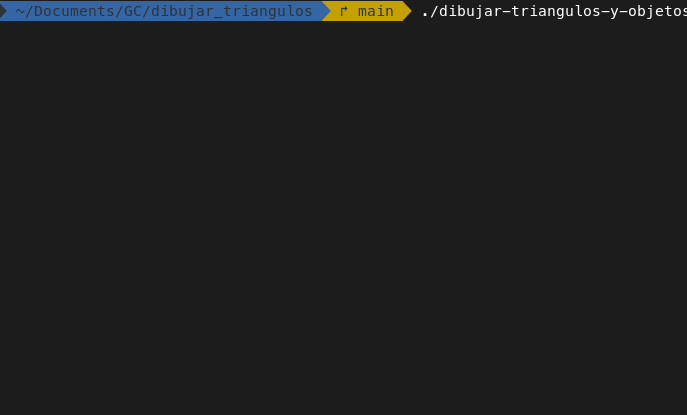
\includegraphics[scale=0.5]{llamada.png}
	\end{minipage}
	
	\item Si deseamos cambiar el fichero predeterminado, pulsamos la tecla "f" y escogemos el fichero que queramos.
	
	\begin{minipage}{\linewidth}
		\centering
		\includegraphics[scale=0.5]{cambiar_fichero.png}
	\end{minipage}
	
	\item El fichero debe seguir estrictamente este formato:
	
	\begin{minipage}{\linewidth}
		\centering
		\includegraphics[scale=0.25]{formato.png}
		\captionof{figure}{Nótese que cada línea contiene un triángulo, tal y como hemos dicho en la introducción.}
	\end{minipage}
\end{enumerate}
Por último, si deseamos cambiar la imagen del programa, hay que tener en cuenta que para ello deberemos cambiar el formato de la imagen a ppm (Portabol Pixmab). Éste formato representa los valores RGB de cada píxel mediante números que van del 0 al 255.
\section{Código C}
A continuación tenemos el código implementeado para que el programa funcionase. Como veremos, se ha dividido en varias funciones para facilitar el entendimiento, con la falta de eficiencia que ello implica. Ésta es la función principal que debíamos cambiar.
\begin{lstlisting}
	void dibujar_triangulo(triobj *optr, int i)
	{
		hiruki *tptr;
		punto *pgoiptr, *pbeheptr, *perdiptr;
		punto *pgoiptr2, *pbeheptr2, *perdiptr2;
		punto corte1, corte2;
		int start1, star2;
		float t = 1, s = 1, q = 1;
		float decremento_t = 1, decremento_s = 1, decremento_q = 1;
		float c1x, c1z, c1u, c1v, c2x, c2z, c2u, c2v;
		int linea;
		float cambio1, cambio1z, cambio1u, cambio1v, cambio2, cambio2z, 
		cambio2u, cambio2v;
		punto p1, p2, p3;
		
		if (i >= optr->num_triangles)
		return;
		tptr = optr->triptr + i;
		mxp(&p1, optr->mptr->m, tptr->p1);
		mxp(&p2, optr->mptr->m, tptr->p2);
		mxp(&p3, optr->mptr->m, tptr->p3);
		if (lineak == 1)
		{
			glBegin(GL_POLYGON);
			glVertex3d(p1.x, p1.y, p1.z);
			glVertex3d(p2.x, p2.y, p2.z);
			glVertex3d(p3.x, p3.y, p3.z);
			glEnd();
			return;
		}
		
		//Encontramos el punto máximo, mínimo, y medio del triángulo.
		
		encontrar_max_min(tptr, &pgoiptr, &perdiptr, &pbeheptr);
		
		// Llamada a función rellenar triángulo.
		
		rellenar_triangulo(pgoiptr, perdiptr, pbeheptr);
		
	}
\end{lstlisting}
Como podemos ver, en la función que deberíamos estar implementando todo, tan solo hemos puesto dos funciones, veamos de cerca ambas:
\begin{lstlisting}
	void encontrar_max_min(hiruki *tptr, punto **pgoiptr, punto **perdiptr, 
	punto **pbeheptr)
	{
		if (tptr->p1.y > tptr->p2.y)
		{
			if (tptr->p1.y > tptr->p3.y)
			{
				*pgoiptr = &(tptr->p1);
				if (tptr->p2.y > tptr->p3.y)
				{
					*perdiptr = &(tptr->p2);
					*pbeheptr = &(tptr->p3);
				}
				else
				{
					*perdiptr = &(tptr->p3);
					*pbeheptr = &(tptr->p2);
				}
			}
			else
			{
				*pgoiptr = &(tptr->p3);
				*perdiptr = &(tptr->p1);
				*pbeheptr = &(tptr->p2);
			}
		}
		else if (tptr->p2.y > tptr->p3.y)
		{
			*pgoiptr = &(tptr->p2);
			*pbeheptr = &(tptr->p1);
			*perdiptr = &(tptr->p3);
		}
		else
		{
			*pgoiptr = &(tptr->p3);
			*pbeheptr = &(tptr->p1);
			*perdiptr = &(tptr->p2);
		}
	}
\end{lstlisting}
La función "encontrar-max-min" busca, dado un triplete de puntos, el punto con mayor valor de $y$, el número con menor de $y$, y el número intermedio de $y$. Cada punto al que le pertenezca dicha $y$ será guardado en el punto que le corresponde pasado por la función. Una vez terminada, deberíamos tener pbeheptr, pgoiptr y perdiptr correctamente escogidos y listos para enviarlos a la función rellenar triángulos. Este procedimiento está sujeto a cambios, puesto que puede que haya formas más simples de enconrar dichos puntos, aunque de momento lo dejaremos así.
\begin{lstlisting}
	void rellenar_triangulo(punto *pgoiptr, punto *perdiptr, punto *pbeheptr)
	{
		int i;
		punto corte1;
		punto corte2;
		
		//Dibujamos la mitad superior del triángulo.
		for (i = pgoiptr->y; i > perdiptr->y; i--)
		{
			calcula_punto_corte(pgoiptr, pbeheptr, i, &corte1);
			calcula_punto_corte(pgoiptr, perdiptr, i, &corte2);
			if (corte1.x <= corte2.x)
			dibujar_linea_z(i, corte1.x, corte1.z, corte1.u, corte1.v, corte2.x, corte2.z, 
			corte2.u, corte2.v);
			else
			dibujar_linea_z(i, corte2.x, corte2.z, corte2.u, corte2.v, corte1.x, corte1.z, 
			corte1.u, corte1.v);
		}
		
		//Dibujamos la mitad inferior del triángulo.
		for (i = perdiptr->y; i > pbeheptr->y; i--)
		{
			calcula_punto_corte(perdiptr, pbeheptr, i, &corte1);
			calcula_punto_corte(pgoiptr, pbeheptr, i, &corte2);
			if (corte1.x <= corte2.x)
			dibujar_linea_z(i, corte1.x, corte1.z, corte1.u, corte1.v, corte2.x, corte2.z, 
			corte2.u, corte2.v);
			else
			dibujar_linea_z(i, corte2.x, corte2.z, corte2.u, corte2.v, corte1.x, corte1.z, 
			corte1.u, corte1.v);
		}
	}
\end{lstlisting}
Ésta es la función más importante, pues se encarga de dibujar el triángulo y ponerle la textura de la imagen ppm que escojamos. Podríamos dividir esta función en dos partes: en el primer bucle, se pinta la mitad superior del triángulo, y en el segundo bucle, se dibujar la mitad inferior del ángulo. Para la primera, escogemos el punto más alto del polígono y se lo asignamos a la variable que vamos a iterar, llamémoslo $i$; ésta la vamos a ir decrementeando en uno hasta que sea menor que el punto medio. Por cada iteración calculamos el punto de corte entre las líneas que unen el punto superior con el punto inferior y medio a dicha altura por medio de calcular-punto-corte. Una vez obtenidos los dos puntos de corte, llamamos a la función dibujar-linea-z y le ofrecemos ambos puntos, junto con la altura a la que queremos situarlo, es decir, $i$. A continuación, se irá ilustrando la línea píxel a píxel. Como veremos, es esta última función que hemos mencionado la que se encarga de obtener el píxel correspondiente de la imagen que pongamos, lo veremos más adelante.
\begin{lstlisting}
	void calcula_punto_corte(punto *punto_superior, punto *punto_inferior, int i, punto *corte)
	{
		float m = 0, m2 = 0, m3 = 0, m4 = 0;
		
		m = (punto_inferior->y - punto_superior->y) / (punto_inferior->x - punto_superior->x);
		m2 = (punto_inferior->y - punto_superior->y) / (punto_inferior->u - punto_superior->u);
		m3 = (punto_inferior->y - punto_superior->y) / (punto_inferior->v - punto_superior->v);
		m4 = (punto_inferior->y - punto_superior->y) / (punto_inferior->z - punto_superior->z);
		corte->x = ((i - punto_superior->y) / m) + punto_superior->x;
		corte->u = ((i - punto_superior->y) / m2) + punto_superior->u;
		corte->v = ((i - punto_superior->y) / m3) + punto_superior->v;
		corte->z = ((i - punto_superior->y) / m4) + punto_superior->z;
	}
\end{lstlisting}
"calcular-punto-corte", tal como dice su nombre, encuentra los puntos de corte que deseamos entre dos puntos y una altura i. Para ello, calculamos la diferencia $\bigtriangleup y$ y la dividimos por la diferencia del punto que queremos encontrar, por ejemplo, $\bigtriangleup x$. Dividimos ambas obteniendo $m$, y finalmente así obtenemos el corte de $x$ gracias a la ecuación de la recta. Repetimos este mismo proceso para cada punto y guardamos su valor en la variable "corte" que se nos pasa por parámetro. 
\begin{lstlisting}
	void dibujar_linea_z(int linea, float c1x, float c1z, float c1u, float c1v, float c2x, 
	float c2z, float c2u, float c2v)
	{
		float xkoord, zkoord;
		float u, v;
		float difu, difv, difz, difx;
		unsigned char r, g, b;
		unsigned char *colorv;
		
		glBegin(GL_POINTS);
		
		//Calculamos la pendiente de la recta que corta el triángulo, si c1x - c2x = 0 evitamos  
		//dividir por cero.
		difx = c1x - c2x;
		if (difx != 0)
		{
			difv = (c2v - c1v) / (difx);
			difu = (c2u - c1u) / (difx);
			difz = (c2z - c2z) / (difx);
		}
		else
		{
			difv = 0;
			difu = 0;
			difz = 0;
		}
		
		for (xkoord = c1x, zkoord = c1z, u = c1u, v = c1v; xkoord <= c2x; xkoord++)
		{
			// TODO
			// color_textura funtzioa ondo kodetu
			
			colorv = color_textura(u, v);
			r = colorv[0];
			g = colorv[1];
			b = colorv[2];
			glColor3ub(r, g, b);
			glVertex3f(xkoord, linea, zkoord);
			// TODO
			// zkoord, u eta v berriak kalkulatu eskuineko puntuarentzat
			// calcular zkoord, u y v del siguiente pixel
			u += difu;
			v += difv;
			zkoord += difz;
		}
		glEnd();
	}
\end{lstlisting}
Éste procedimiento sigue el mismo principio aritmético que calcular-punto-corte sigue. A dibujar-linea se le pasan los puntos de corte $x_1$, $y_1$, .... Teniendo en cuenta que el primer punto se encuentra más a la izquierda en el plano cartesiano que el segundo. Primero de todo calculamos $\bigtriangleup x$, y nos aseguramos de que la diferencia entre ambos no sea cero, si se cumple, calculamos la diferencia del punto del que queramos obtener la pendiente, por ejemplo, $\bigtriangleup u$, y lo dividimos. En el caso de que $\bigtriangleup x$ sea cero, evitamos dividir y asignamos cero a difv, difu y difz. Así, una vez entramos en el bucle, ya tenemos todo lo necesario, puesto que cada iteración sumamos a tanto u, v como zkoord la diferencia que hemos obtenido para ir moviéndonos más y más hacia la derecha mientras dibujamos píxel tras píxel: En definitiva, estamos haciendo uso del algoritmo de Brassenham en coma flotante para dibujar rectas. Puede haber espacio para mejora, dado que el algoritmo con enteros es más eficiente, y ajustándolo obtendríamos una mayor eficiencia. 
Para pintar cada punto y saber el color que le corresponde, llamamos a color-textura, que le pasamos los puntos correspondientes $(u,v)$  de la imagen que hemos escogido para que calcules sus valores RGB.
\begin{lstlisting}
	unsigned char *color_textura(float u, float v)
	{
		char *lag;
		
		int desplazamiento_u, desplazamiento_v;
		
		desplazamiento_u = trunc (u * dimx);
		desplazamiento_v = trunc ((1-v)*dimy);
		
		lag = (unsigned char *)bufferra; // pixel on the left and top
		return (lag + 3 * (desplazamiento_v * dimx + desplazamiento_u));
	}
\end{lstlisting}
Para terminar, hemos modificado la función color-textura para que se desplazase correctamente hacia el píxel de la imagen. No hay mucho que explicar, salvo que tenemos que restar v por uno dado que nos tenemos que desplazar esas casillas para acceder a la casilla correcta.
\section{Trabajo futuro}
Principalmente, lo más importante será buscar una mejora de eficiencia en la aplicación, quizá cambiando la forma en que la llamada a las funciones está pensada, o usando algoritmos que no requieran tantos flops como este lo hace. 
\end{document}
